%Section 1
\section{Pary}

\textbf{Parę uporządkowaną} (lub po prostu \textbf{parę}) zapisywać będziemy w postaci \m{ \pair{a}{b} }. Para jest jednym z \textbf{pojęć pierwotnych}. Przyjmiemy, że para spełnia następujący aksjomat:
\begin{axiom}
\m{ \pair{a}{b} = \pair{c}{d} } wtedy i tylko wtedy, gdy \m{ a = c } oraz \m{ b = d }.
\end{axiom}

Aksjomat ten mówi, że dwie pary są równe, jeśli są równe zarówno na pierwszym jak i na drugim elemencie. To znaczy, że pary \m{ \pair{1}{2} } i \m{ \pair{1}{3} } nie są równe (bo są różne na drugim elemencie), natomiast pary \m{ \pair{1}{2} } oraz \m{ \pair{1}{2} } są.

Zbiór wszystkich par, których pierwszy element pochodzi z jakiegoś zbioru \m{A} a drugi z jakiegoś zbioru \m{B} nazywać będziemy \textbf{iloczynem kartezjańskim} i zapisywać jako \m{ A \times B }. Formalnie:

\[
    A \times B = \set{\pair{a}{b}}{a \in A \wedge b \in B}
\]

Dla przykładu, dla zbiorów \m{A = \{ 1,2 \} } oraz \m{B = \{ 3,4 \} }, iloczyn kartezjański \m{ A \times B }  to zbiór \m{\{ 1,2 \} \times \{ 3,4 \} = \{ \pair{1}{3}, \pair{1}{4}, \pair{2}{3}, \pair{2}{4} \} }.

\begin{ex}
Zapisz iloczyny kartezjańskie poniższych zbiorów:
\begin{itemize}
    \item \({ A = \{ 1 \} }\),~\({ B = \{ 1,2 \} }\)
    \item \({ A = \{ 1,2 \} }\),~\({ B = \{ 1,2 \} }\)
    \item \({ A = \emptyset }\),~\({ B = \{ 1,2 \} }\)
    \item \({ A = \{ 1,2 \} }\),~\({ B = \emptyset }\)
    \item \({ A = \emptyset }\),~\({ B = \emptyset }\)
\end{itemize}
\end{ex}

Czasem, zamiast pisać \m{A \times A} (zbiór wszystkich par w których zarówno pierwszy jak i drugi element pochodzą ze zbioru \m{A}) będziemy pisać \m{A^2}.

Przyjrzyjmy się teraz poniższej równości:

\[
    \underbrace{(A \cap B) \times C}_{L} = \underbrace{(A \times C) \cap (B \times C)}_{P} 
\]

Jak stwierdzić, czy jest ona prawdziwa?

Zarówno \m{L} jak i \m{P} są \textbf{zbiorami}. Wiemy, że są one równe, jeśli dla dowolnego elementu \m{z \in L }, \m{z \in P } oraz dla dowolnego elementu \m{z \in P }, \m{ z \in L }. Elementami zarówno zbioru \m{L} jak i zbioru \m{P} są \textbf{pary}. Weźmy więc dowolną parę \m{ \pair{x}{y} \in L }

\[ 
\begin{split}
        \pair{x}{y} \in L
        & \equiv \pair{x}{y} \in (A \cap B) \times C 
        \\& \stackrel{(1)}{\equiv} x \in (A \cap B) \wedge y \in C
        \\& \stackrel{(2)}{\equiv} x \in A \wedge x \in B \wedge y \in C
\end{split}
\]

Przejście \m{(1)} wynika wprost z definicji \textbf{iloczynu kartezjańskiego} który poznaliśmy w tym rozdziale: para \m{ \pair{x}{y} } należy do iloczynu kartezjańskiego \m{ (A \cap B) \times C }, z definicji wtedy i tylko wtedy gdy \m{x} należy do \m{A \cap B}, a \m{y} należy do \m{C}. Przejście \m{(2)} wynika z definicji przekroju zbiorów, którą już znamy.

Weźmy teraz dowolną parę \m{\pair{x}{y} \in P }

\[
\begin{split}
    \pair{x}{y} \in P
    & \equiv \pair{x}{y} \in (A \times C) \cap (B \times C) 
    \\& \stackrel{(1)}{\equiv} \pair{x}{y} \in (A \times C) \wedge \pair{x}{y} \in (B \times C) 
    \\& \stackrel{(2)}{\equiv} x \in A \wedge y \in C \wedge x \in B \wedge y \in C 
    \\& \stackrel{(3)}{\equiv} x \in A \wedge y \in C \wedge x \in B 
    \\& \stackrel{(4)}{\equiv} x \in A \wedge y \in B \wedge x \in C
    \\& \stackrel{(5)}{\equiv} x \in (A \cap B) \wedge y \in C
    \\& \stackrel{(6)}{\equiv}  \pair{x}{y} \in (A \cap B) \times C \equiv \pair{x}{y} \in L
\end{split}
\]

Przejście \m{(1)} wynika z definicji przekroju zbiorów, przejście \m{(2)} wynika z definicji iloczynu kartezjańskiego, przejścia \m{(3)} oraz \m{(4)} wynikają z własności formuł rachunku zdań~(\m{\varphi \wedge \varphi \equiv \varphi} oraz przemienność koniunkcji) natomiast przejścia \m{(5)} i \m{(6)} rozpisaliśmy wyżej.

Możemy z tego wywnioskować, że \m{pair{x}{y} \in L \equiv \pair{x}{y} \in P}. Skoro napisy te są równoważne, to dowolny element należący do \m{L} należy też do \m{P}, a dowolny element należący do \m{P} należy też do \m{L}. To oznacza, że zbiory \m{L} oraz \m{P} są równe, więc równość

\[
    \underbrace{(A \cap B) \times C}_{L} = \underbrace{(A \times C) \cap (B \times C)}_{P} 
\]

Jest prawdziwa.

%Section 2
\section{Relacje}

\textbf{Relacją} binarną (lub dwuargumentową) nazywać będziemy dowolny zbiór \textbf{par}, których pierwszy element należy do zbioru \m{A}, a drugi element do zbioru \m{B}. Bardziej formalnie:

\begin{definition}[Relacja binarna]
Relacją binarną (dwuargumentową) nazywamy dowolny podzbiór \m{R \subseteq A \times B}.
\end{definition}

Elementy \m{a} i \m{b} są \textbf{w relacji \m{R}}, jeśli para \m{\pair{a}{b}} jest elementem zbioru \m{R}. Podzbiory \m{A\times A} (czyli zbiory par z których zarówno pierwszy jak i drugi element pochodzą ze zbioru \m{A}), nazywamy \textbf{relacjami binarnymi na zbiorze \m{A}}.

Przykładem relacji może być znana nam relacja \textbf{mniejszości} na zbiorze liczb naturalnych (\m{\set{\pair{x}{y} \in \mathbb{N}^2}{x < y}}): liczby naturalne \m{x} i \m{y} są w relacji (\m{xRy})), jeśli \m{x} jest \textbf{mniejsze} niż \m{y}. Relacją jest także relacja \textbf{identyczności} na zbiorze liczb naturalnych (\m{I_{\mathbb{N}} = \set{\pair{x}{x} \in \mathbb{N}^2}{x \in \mathbb{N}}}): każda liczba naturalna jest w relacji jedynie z samą sobą (\m{xRx} dla każdej liczby naturalnej). Inną relacją jest relacja \textbf{bycia kwadratem} (\m{\set{\pair{x}{y} \in \mathbb{Z}\times \mathbb{N}}{y = x^2}}): dowolna liczba całkowita \m{x} jest w relacji z liczbą naturalną, będącą kwadratem liczby \m{x}.

Relację binarną na zbiorze \m{A} (to znaczy relację \m{R \subseteq A\times A}) wyobrażać sobie można jako \textbf{graf skierowany}: zbiór \textbf{wierzchołków} (reprezentujących elementy zbioru \m{A}), które mogą być połączone \textbf{krawędziami} (reprezentującymi relację) tak, że każda krawędź zaczyna się i kończy w jakimś wierzchołku.

Przykładowo, rozpatrzmy relację mniejszości na zbiorze \m{\{ 1,2,3 \} }, to znaczy \m{R = \set{\pair{x}{y} \in \{ 1,2,3 \}^2}{x < y}}, czyli zbiór par \m{\{ \pair{1}{2}, \pair{1}{3}, \pair{2}{3} \}}. Relację tą możemy sobie wyobrażać jako następujący graf:

\begin{center}
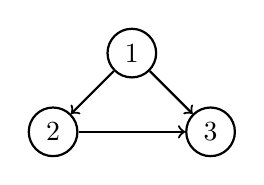
\begin{tikzpicture}
\begin{scope}[every node/.style={circle,thick,draw}]
    \node (A) at (1,1) {\m{1}};
    \node (B) at (0,0) {\m{2}};
    \node (C) at (2,0) {\m{3}};
\end{scope}
\begin{scope}[every edge/.style={draw=black,thick}]
    \path[->] (A) edge (B);
    \path[->] (A) edge (C);
    \path[->] (B) edge (C);
\end{scope}
\end{tikzpicture}
\end{center}

Podobnie możemy przedstawić relację identyczności na tym samym zbiorze: \m{I_{\{ 1,2,3 \}} = \set{\pair{x}{x} \in \{ 1,2,3 \}^2}{x \in \{1,2,3 \}}}, czyli zbiór par \m{ \{ \pair{1}{1}, \pair{2}{2}, \pair{3}{3} \} }. Tą relację możemy sobie wyobrażać jako następujący graf:

\begin{center}
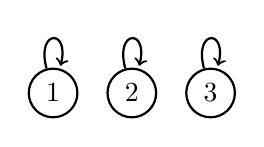
\begin{tikzpicture}
\begin{scope}[every node/.style={circle,thick,draw}]
    \node (A) at (0,0) {\m{1}};
    \node (B) at (1,0) {\m{2}};
    \node (C) at (2,0) {\m{3}};
\end{scope}
\begin{scope}[every edge/.style={draw=black,thick}]
    \path[->] (A) edge [loop above] (A);
    \path[->] (B) edge [loop above] (B);
    \path[->] (C) edge [loop above] (C);
\end{scope}
\end{tikzpicture}
\end{center}

Relacje na dowolnym zbiorze \m{A} (czyli relacje \m{R \subseteq A \times A}) mogą posiadać różne własności:

\begin{definition}
Relacja \m{R \subseteq A \times A} jest:
\begin{itemize}
    \item \textbf{zwrotna}, jeśli dla wszystkich \m{a \in A} zachodzi \m{aRa} (czyli dla każdego \m{a}, \m{a} jest w relacji z samym sobą).
    \item \textbf{symetryczna}, jeśli dla wszystkich \m{a,b \in A}, jeśli \m{aRb}, to \m{bRa} (czyli dla każdych \m{a,b} jeśli \m{a} jest w relacji z \m{b}, to \m{b} jest w relacji z \m{a}).
    \item \textbf{przechodnia}, jeśli dla wszystkich \m{a,b,c \in A}, jeśli \m{aRb} oraz \m{bRc}, to \m{aRc} (czyli dla każdych \m{a,b,c} jeśli \m{a} jest w relacji z \m{b} i \m{b} jest w relacji z \m{c}, to \m{a} jest w relacji z \m{c}).
    \item \textbf{antyzwrotna}, jeśli dla każdego \m{a}, \textbf{nie} zachodzi \m{aRa} (czyli dla każdego \m{a}, \m{a} nie jest w relacji z \m{a}).
    \item \textbf{antysymetryczna}, jeśli dla wszystkich \m{a,b}, jeśli \m{aRb}, to nie zachodzi \m{bRa} (czyli, dla dowolnych \m{a,b}, jeśli \m{a} jest w relacji z \m{b}, to \m{b} nie jest w relacji z \m{a}).
    \item \textbf{słabo antysymetryczna}, jeśli dla wszystkich \m{a,b}, jeśli \m{aRb} oraz \m{bRa}, to \m{a = b} (czyli, dla dowolnych \m{a,b}, jeśli \m{a} jest w relacji z \m{b}, oraz \m{b} jest w relacji z \m{a}, to \m{a} jest równie \m{b}).
\end{itemize}
\end{definition}

Poniżej przedstawiamy graficzne (grafowe) zobrazowanie podanych wyżej definicji:

\begin{itemize}
    \item Relacja jest zwrotna, jeśli dla każdego \m{a \in A} zachodzi \m{aRa}. W przypadku grafu oznacza to, że każdy element ma krawędź do samego siebie. Poniższe relacje są przykładami relacji zwrotnych:
\begin{center}
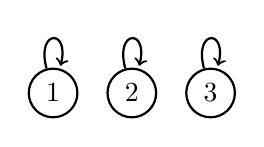
\begin{tikzpicture}
\begin{scope}[every node/.style={circle,thick,draw}]
    \node (A) at (0,0) {\m{1}};
    \node (B) at (1,0) {\m{2}};
    \node (C) at (2,0) {\m{3}};
\end{scope}
\begin{scope}[every edge/.style={draw=black,thick}]
    \path[->] (A) edge [loop above] (A);
    \path[->] (B) edge [loop above] (B);
    \path[->] (C) edge [loop above] (C);
\end{scope}
\end{tikzpicture}
\end{center}

\begin{center}
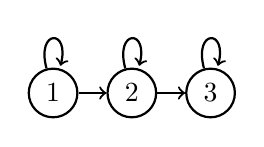
\begin{tikzpicture}
\begin{scope}[every node/.style={circle,thick,draw}]
    \node (A) at (0,0) {\m{1}};
    \node (B) at (1,0) {\m{2}};
    \node (C) at (2,0) {\m{3}};
\end{scope}
\begin{scope}[every edge/.style={draw=black,thick}]
    \path[->] (A) edge [loop above] (A)
                  edge              (B);
    \path[->] (B) edge [loop above] (B)
                  edge              (C);
    \path[->] (C) edge [loop above] (C);
\end{scope}
\end{tikzpicture}
\end{center}

\begin{center}
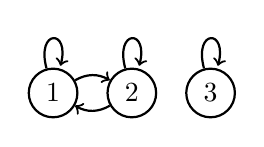
\begin{tikzpicture}
\begin{scope}[every node/.style={circle,thick,draw}]
    \node (A) at (0,0) {\m{1}};
    \node (B) at (1,0) {\m{2}};
    \node (C) at (2,0) {\m{3}};
\end{scope}
\begin{scope}[every edge/.style={draw=black,thick}]
    \path[->] (A) edge [loop above] (A)
                   edge [bend left] (B);
    \path[->] (B) edge [loop above] (B)
                  edge [bend left] (A);
    \path[->] (C) edge [loop above] (C);
\end{scope}
\end{tikzpicture}
\end{center}

z kolei 
\begin{center}
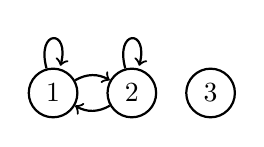
\begin{tikzpicture}
\begin{scope}[every node/.style={circle,thick,draw}]
    \node (A) at (0,0) {\m{1}};
    \node (B) at (1,0) {\m{2}};
    \node (C) at (2,0) {\m{3}};
\end{scope}
\begin{scope}[every edge/.style={draw=black,thick}]
    \path[->] (A) edge [loop above] (A)
                   edge [bend left] (B);
    \path[->] (B) edge [loop above] (B)
                  edge [bend left] (A);
\end{scope}
\end{tikzpicture}
\end{center}
relacją zwrotną nie jest (ponieważ \m{3} nie jest w relacji z \m{3}).

\item Relacja jest symetryczna, jeśli dla każdego \m{a,b \in A}, jeśli \m{aRb} to \m{bRa}. W przypadku grafu oznacza to, że dla dowolnych elementów, jeśli istnieje krawędż z jednego do drugiego, to istnieje także krawędź w drugą stronę. Przykładowo, poniższe relacje są symetryczne:

\begin{center}
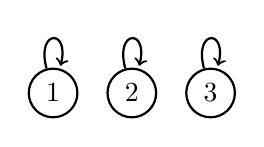
\begin{tikzpicture}
\begin{scope}[every node/.style={circle,thick,draw}]
    \node (A) at (0,0) {\m{1}};
    \node (B) at (1,0) {\m{2}};
    \node (C) at (2,0) {\m{3}};
\end{scope}
\begin{scope}[every edge/.style={draw=black,thick}]
    \path[->] (A) edge [loop above] (A);
    \path[->] (B) edge [loop above] (B);
    \path[->] (C) edge [loop above] (C);
\end{scope}
\end{tikzpicture}
\end{center}

\begin{center}
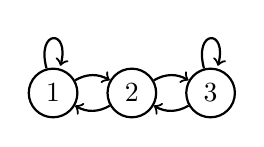
\begin{tikzpicture}
\begin{scope}[every node/.style={circle,thick,draw}]
    \node (A) at (0,0) {\m{1}};
    \node (B) at (1,0) {\m{2}};
    \node (C) at (2,0) {\m{3}};
\end{scope}
\begin{scope}[every edge/.style={draw=black,thick}]
    \path[->] (A) edge [loop above] (A)
                  edge [bend left] (B);
    \path[->] (B) edge [bend left] (A) 
                  edge [bend left] (C);
    \path[->] (C) edge [loop above] (C)
                  edge [bend left] (B);
\end{scope}
\end{tikzpicture}
\end{center}

\begin{center}
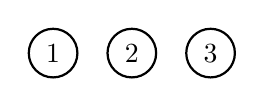
\begin{tikzpicture}
\begin{scope}[every node/.style={circle,thick,draw}]
    \node (A) at (0,0) {\m{1}};
    \node (B) at (1,0) {\m{2}};
    \node (C) at (2,0) {\m{3}};
\end{scope}
\end{tikzpicture}
\end{center}

z kolei

\begin{center}
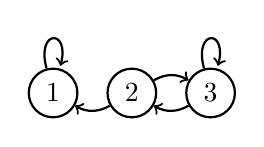
\begin{tikzpicture}
\begin{scope}[every node/.style={circle,thick,draw}]
    \node (A) at (0,0) {\m{1}};
    \node (B) at (1,0) {\m{2}};
    \node (C) at (2,0) {\m{3}};
\end{scope}
\begin{scope}[every edge/.style={draw=black,thick}]
    \path[->] (A) edge [loop above] (A);
    \path[->] (B) edge [bend left] (A) 
                  edge [bend left] (C);
    \path[->] (C) edge [loop above] (C)
                  edge [bend left] (B);
\end{scope}
\end{tikzpicture}
\end{center}

nie jest relacją symetryczną -- elementy \m{1} i \m{2} są w relacji, natomiast \m{2} i \m{1} nie są. Podobnie

\begin{center}
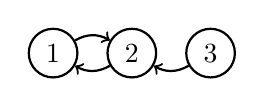
\begin{tikzpicture}
\begin{scope}[every node/.style={circle,thick,draw}]
    \node (A) at (0,0) {\m{1}};
    \node (B) at (1,0) {\m{2}};
    \node (C) at (2,0) {\m{3}};
\end{scope}
\begin{scope}[every edge/.style={draw=black,thick}]
    \path[->] (A) edge [bend left] (B);
    \path[->] (B) edge [bend left] (A);
    \path[->] (C) edge [bend left] (B);
\end{scope}
\end{tikzpicture}
\end{center}

nie jest relacją symetryczną, bo elementy \m{3} i \m{2} są w relacji, a \m{2} i \m{3} nie są.

\item Relacja jest przechodnia, jeśli dla wszystkich \m{a,b,c \in A}, jeśli \m{aRb} i \m{bRc} to \m{aRc}. W przypadku grafów oznacza to, że jeśli z jakiegoś wierzchołka do innego potrafię dotrzeć w dwóch krokach, to powinienem też móc tam dotrzeć w jednym kroku. Poniższe relacje są przykładami relacji przechodnich:

\begin{center}
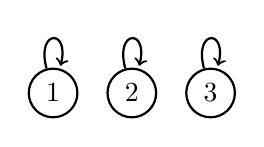
\begin{tikzpicture}
\begin{scope}[every node/.style={circle,thick,draw}]
    \node (A) at (0,0) {\m{1}};
    \node (B) at (1,0) {\m{2}};
    \node (C) at (2,0) {\m{3}};
\end{scope}
\begin{scope}[every edge/.style={draw=black,thick}]
    \path[->] (A) edge [loop above] (A);
    \path[->] (B) edge [loop above] (B);
    \path[->] (C) edge [loop above] (C);
\end{scope}
\end{tikzpicture}
\end{center}

\begin{center}
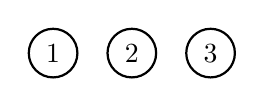
\begin{tikzpicture}
\begin{scope}[every node/.style={circle,thick,draw}]
    \node (A) at (0,0) {\m{1}};
    \node (B) at (1,0) {\m{2}};
    \node (C) at (2,0) {\m{3}};
\end{scope}
\end{tikzpicture}
\end{center}

\begin{center}
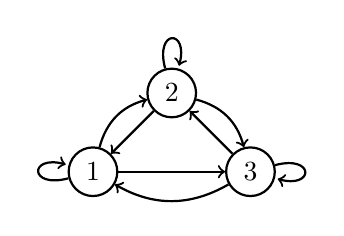
\begin{tikzpicture}
\begin{scope}[every node/.style={circle,thick,draw}]
    \node (A) at (0,0) {\m{1}};
    \node (B) at (1,1) {\m{2}};
    \node (C) at (2,0) {\m{3}};
\end{scope}
\begin{scope}[every edge/.style={draw=black,thick}]
    \path[->] (A) edge [loop left] (A)
                  edge [bend left] (B)
                  edge [left] (C);
    \path[->] (B) edge [loop above] (B)
                  edge [left] (A)
                  edge [bend left] (C);
    \path[->] (C) edge [loop right] (C)
                  edge [bend left] (A)
                  edge [left] (B);
\end{scope}
\end{tikzpicture}
\end{center}

z kolei 

\begin{center}
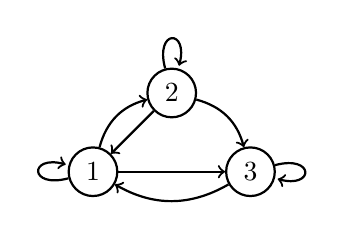
\begin{tikzpicture}
\begin{scope}[every node/.style={circle,thick,draw}]
    \node (A) at (0,0) {\m{1}};
    \node (B) at (1,1) {\m{2}};
    \node (C) at (2,0) {\m{3}};
\end{scope}
\begin{scope}[every edge/.style={draw=black,thick}]
    \path[->] (A) edge [loop left] (A)
                  edge [bend left] (B)
                  edge [left] (C);
    \path[->] (B) edge [loop above] (B)
                  edge [left] (A)
                  edge [bend left] (C);
    \path[->] (C) edge [loop right] (C)
                  edge [bend left] (A);
\end{scope}
\end{tikzpicture}
\end{center}

relacją przechodnią nie jest -- \m{3} jest w relacji z \m{1} (pierwszy krok), \m{1} jest w relacji z \m{2} (drugi krok), ale \m{3} nie jest w relacji z \m{2} (czyli z \m{3} do \m{2} możemy dotrzeć w dwóch krokach, ale nie możemy dotrzeć w jednym). Relacja 

\begin{center}
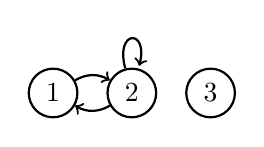
\begin{tikzpicture}
\begin{scope}[every node/.style={circle,thick,draw}]
    \node (A) at (0,0) {\m{1}};
    \node (B) at (1,0) {\m{2}};
    \node (C) at (2,0) {\m{3}};
\end{scope}
\begin{scope}[every edge/.style={draw=black,thick}]
    \path[->] (A) edge [bend left] (B);
    \path[->] (B) edge [loop above] (B)
                  edge [bend left] (A);
\end{scope}
\end{tikzpicture}
\end{center}

również \textbf{nie jest} przechodnia -- \m{1} jest w relacji z \m{2} (pierwszy krok) a \m{2} jest w relacji z \m{1}, ale \m{1} nie jest w relacji z \m{1} (z \m{1} do \m{1} mogę dotrzeć w dwóch krokach, ale nie mogę dotrzeć w jednym).

\item Relacja jest antyzwrotna, jeśli dla każdego \m{a \in A} nie zachodzi \m{aRa}. W przypadku grafu oznacza to, że nie ma elementu który ma krawędź sam do siebie. Poniższe relacje są przykładami relacji antyzwrotnych: 

\begin{center}
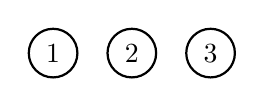
\begin{tikzpicture}
\begin{scope}[every node/.style={circle,thick,draw}]
    \node (A) at (0,0) {\m{1}};
    \node (B) at (1,0) {\m{2}};
    \node (C) at (2,0) {\m{3}};
\end{scope}
\end{tikzpicture}
\end{center}

\begin{center}
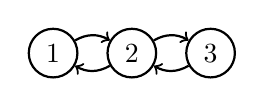
\begin{tikzpicture}
\begin{scope}[every node/.style={circle,thick,draw}]
    \node (A) at (0,0) {\m{1}};
    \node (B) at (1,0) {\m{2}};
    \node (C) at (2,0) {\m{3}};
\end{scope}
\begin{scope}[every edge/.style={draw=black,thick}]
    \path[->] (A) edge [bend left] (B);
    \path[->] (B) edge [bend left] (A) 
                  edge [bend left] (C);
    \path[->] (C) edge [bend left] (B);
\end{scope}
\end{tikzpicture}
\end{center}

z kolei relacja

\begin{center}
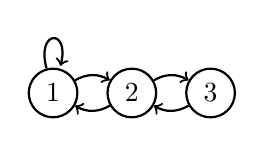
\begin{tikzpicture}
\begin{scope}[every node/.style={circle,thick,draw}]
    \node (A) at (0,0) {\m{1}};
    \node (B) at (1,0) {\m{2}};
    \node (C) at (2,0) {\m{3}};
\end{scope}
\begin{scope}[every edge/.style={draw=black,thick}]
    \path[->] (A) edge [loop above] (A)
                  edge [bend left] (B);
    \path[->] (B) edge [bend left] (A) 
                  edge [bend left] (C);
    \path[->] (C) edge [bend left] (B);
\end{scope}
\end{tikzpicture}
\end{center}

antyzwrotna nie jest, ponieważ \m{1} jest w relacji z samą sobą (\m{1} ma strzałkę do samego siebie).

\item Relacja jest antysymetryczna, jeśli dla wszystkich \m{a,b \in A}, jeśli \m{aRb} to nie zachodzi \m{bRa}. W przypadku grafów oznacza to, że jeśli istnieje krawędź w jedną stronę, to nie istnieje krawędź w drugą. Ponosze relacje są przykładami relacji antysymetrycznych:

\begin{center}
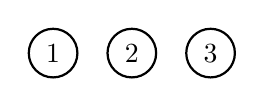
\begin{tikzpicture}
\begin{scope}[every node/.style={circle,thick,draw}]
    \node (A) at (0,0) {\m{1}};
    \node (B) at (1,0) {\m{2}};
    \node (C) at (2,0) {\m{3}};
\end{scope}
\end{tikzpicture}
\end{center}

\begin{center}
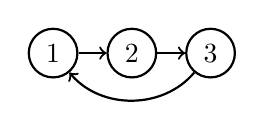
\begin{tikzpicture}
\begin{scope}[every node/.style={circle,thick,draw}]
    \node (A) at (0,0) {\m{1}};
    \node (B) at (1,0) {\m{2}};
    \node (C) at (2,0) {\m{3}};
\end{scope}
\begin{scope}[every edge/.style={draw=black,thick}]
    \path[->] (A) edge [left] (B);
    \path[->] (B) edge [left] (C);
    \path[->] (C) edge [bend left=50] (A);
\end{scope}
\end{tikzpicture}
\end{center}

z kolei relacja 

\begin{center}
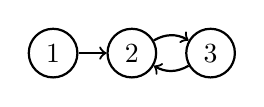
\begin{tikzpicture}
\begin{scope}[every node/.style={circle,thick,draw}]
    \node (A) at (0,0) {\m{1}};
    \node (B) at (1,0) {\m{2}};
    \node (C) at (2,0) {\m{3}};
\end{scope}
\begin{scope}[every edge/.style={draw=black,thick}]
    \path[->] (A) edge [left] (B);
    \path[->] (B) edge [bend left] (C);
    \path[->] (C) edge [bend left] (B);
\end{scope}
\end{tikzpicture}
\end{center}

antysymetryczna nie jest -- \m{2} jest w relacji z \m{3} oraz \m{3} jest w relacji z \m{2}. Relacja 

\begin{center}
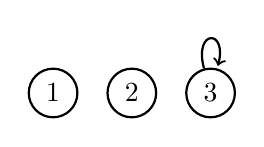
\begin{tikzpicture}
\begin{scope}[every node/.style={circle,thick,draw}]
    \node (A) at (0,0) {\m{1}};
    \node (B) at (1,0) {\m{2}};
    \node (C) at (2,0) {\m{3}};
\end{scope}
\begin{scope}[every edge/.style={draw=black,thick}]
    \path[->] (C) edge [loop above] (C);
\end{scope}
\end{tikzpicture}
\end{center}

także nie jest antysymetryczna -- \m{3} jest w relacji z \m{3} oraz \m{3} jest w relacji z \m{3} (dla \textbf{każdych} \m{a, b} jeśli \m{aRb}, to nie może zachodzić \m{bRa} -- skoro dla każdych, to w szczególności dla \m{a=b=3}).

\item Relacja jest słabo antysymetryczna, jeśli dla wszystkich \m{a,b \in A}, jeśli \m{aRb} i \m{bRa}, to \m{a=b}. Zauważmy, że dowolna relacja antysymetryczna jest też słabo antysymetryczna. W przypadku grafu oznacza to więc, że jeśli istnieje krawędź w jedną stronę, to nie istnieje krawędź w drugą, \textbf{chyba, że} jest to ,,pętla'' (krawędź z wierzchołka do jego samego, czyli \m{aRa}). Relacje 

\begin{center}
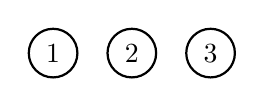
\begin{tikzpicture}
\begin{scope}[every node/.style={circle,thick,draw}]
    \node (A) at (0,0) {\m{1}};
    \node (B) at (1,0) {\m{2}};
    \node (C) at (2,0) {\m{3}};
\end{scope}
\end{tikzpicture}
\end{center}

\begin{center}
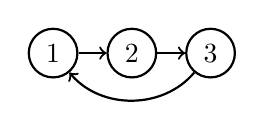
\begin{tikzpicture}
\begin{scope}[every node/.style={circle,thick,draw}]
    \node (A) at (0,0) {\m{1}};
    \node (B) at (1,0) {\m{2}};
    \node (C) at (2,0) {\m{3}};
\end{scope}
\begin{scope}[every edge/.style={draw=black,thick}]
    \path[->] (A) edge [left] (B);
    \path[->] (B) edge [left] (C);
    \path[->] (C) edge [bend left=50] (A);
\end{scope}
\end{tikzpicture}
\end{center}

są słabo antysymetryczne (ponieważ są też antysymetryczne). Dodatkowo, relacja 

\begin{center}
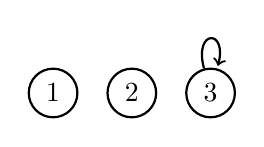
\begin{tikzpicture}
\begin{scope}[every node/.style={circle,thick,draw}]
    \node (A) at (0,0) {\m{1}};
    \node (B) at (1,0) {\m{2}};
    \node (C) at (2,0) {\m{3}};
\end{scope}
\begin{scope}[every edge/.style={draw=black,thick}]
    \path[->] (C) edge [loop above] (C);
\end{scope}
\end{tikzpicture}
\end{center}

która, jak ustaliliśmy wcześniej, antysymetryczna nie jest, jest słabo antysymetryczna. Relacja 

\begin{center}
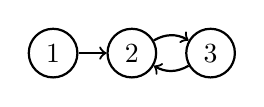
\begin{tikzpicture}
\begin{scope}[every node/.style={circle,thick,draw}]
    \node (A) at (0,0) {\m{1}};
    \node (B) at (1,0) {\m{2}};
    \node (C) at (2,0) {\m{3}};
\end{scope}
\begin{scope}[every edge/.style={draw=black,thick}]
    \path[->] (A) edge [left] (B);
    \path[->] (B) edge [bend left] (C);
    \path[->] (C) edge [bend left] (B);
\end{scope}
\end{tikzpicture}
\end{center}

nie jest jednak słabo antysymetryczna -- \m{2} jest w relacji z \m{3} i \m{3} jest w relacji z \m{2}, jednak \m{2 \neq 3} (istnieje krawędź w jedną i w drugą stronę, ale nie jest to krawędź z wierzchołka do samego siebie). 
\end{itemize}

Czy istnieje relacja, która jest zarazem antysymetryczna jak i zwrotna? Wydaje się, że odpowiedź to \textbf{nie} -- skoro każdy element musi mieć krawędź do samego siebie (być w relacji z samym sobą), wyklucza to antysymetryczność. Zaskakująco jednak, odpowiedź brzmi \textbf{tak}. Przykładem takiej relacji jest relacja \textbf{pusta} na zbiorze \textbf{pustym}: relacja, w której nie ma żadnych elementów, nad zbiorem w którym także nie ma żadnych elementów. Taka relacja spełnia wszystkie kryteria bycia relacją (jest zbiorem par), relacji zwrotnej (\textbf{dla każdego} elementu \m{a \in \emptyset}, a wiemy, że taki element nie istnieje) oraz relacji słabo antysymetrycznej (nie ma żadnej krawędzi, więc w szczególności nie zachodzi sytuacja, że jest krawędź w jedną stronę i krawędź w drugą stronę). Analogicznie można myśleć o tym, że nie znajdziemy \textbf{kontrprzykładu} na fakt, że relacja \textbf{jest zwrotna}: żeby relacja nie była zwrotna, musi istnieć wierzchołek, który nie ma krawędzi sam do siebie (czyli istnieć element, który nie jest ze sobą w relacji), jednak takiego elementu nie znajdziemy, ponieważ zbiór, na którym określamy relację, jest pusty.

Relacja pusta na zbiorze pustym jest szczególnym przypadkiem relacji, która spełnia wszystkie powyższe definicje: jest \textbf{przechodnia}, \textbf{zwrotna} i \textbf{antyzwrotna}, \textbf{symetryczna} i \textbf{antysymetryczna} a także \textbf{słabo antysymetryczna}. Zauważmy, że jeśli zbiór, na którym określamy relację, ma przynajmniej jeden element, to spełnienie wszystkich definicji jednocześnie jest niemożliwe: w szczególności, relacja na zbiorze który posiada przynajmniej jeden element nie może być jednocześnie zwrotna i antysymetryczna (ponieważ istnieje element \m{a \in A} taki, że \m{aRa}, ale skoro istnieje takie \m{a}, że \m{aRa}, to z definicji relacja nie jest antysymetryczna). 

\begin{example}
Czy istnieje relacja, która jest zwrotna i symetryczna, ale nie jest przechodnia? 

Spróbujmy zbudować taką relację. Zacznijmy więc od zdefiniowania zbioru \m{A}, na którym będziemy relację określać. Wiemy, z wcześniejszych obserwacji, że dla \m{A = \emptyset} (dla której istnieje tylko jedna relacja -- relacja pusta), relacja będzie symetryczna. Dla zbioru \m{A = \{1\}}, istnieje tylko jedna relacja zwrotna:

\begin{center}
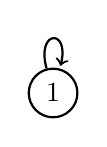
\begin{tikzpicture}
\begin{scope}[every node/.style={circle,thick,draw}]
    \node (A) at (0,0) {\m{1}};
\end{scope}
\begin{scope}[every edge/.style={draw=black,thick}]
    \path[->] (A) edge [loop above] (A);
\end{scope}
\end{tikzpicture}
\end{center}

Powyższa relacja jest jednak przechodnia. W zbiorze \m{\{ 1,2 \}} są tylko cztery relacje zwrotne, jednak wszystkie z nich są przechodnie (łatwo jest rozrysować wszystkie cztery i sprawdzić). Spróbujmy więc rozpatrzeć zbiór \m{\{1,2,3\}}. Wszystkie relacje, które powstaną przez dorysowanie krawędzi do relacji 

\begin{center}
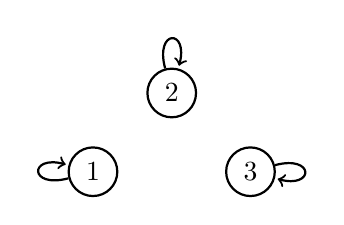
\begin{tikzpicture}
\begin{scope}[every node/.style={circle,thick,draw}]
    \node (A) at (0,0) {\m{1}};
    \node (B) at (1,1) {\m{2}};
    \node (C) at (2,0) {\m{3}};
\end{scope}
\begin{scope}[every edge/.style={draw=black,thick}]
    \path[->] (A) edge [loop left] (A);
    \path[->] (B) edge [loop above] (B);
    \path[->] (C) edge [loop right] (C);
\end{scope}
\end{tikzpicture}
\end{center}

będą zwrotne. Przykładem relacji zwrotnej, która nie jest przechodnia, może być następująca relacja:

\begin{center}
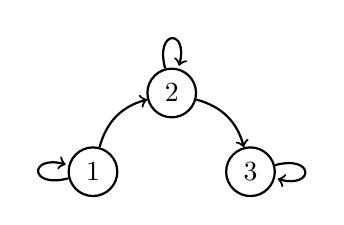
\begin{tikzpicture}
\begin{scope}[every node/.style={circle,thick,draw}]
    \node (A) at (0,0) {\m{1}};
    \node (B) at (1,1) {\m{2}};
    \node (C) at (2,0) {\m{3}};
\end{scope}
\begin{scope}[every edge/.style={draw=black,thick}]
    \path[->] (A) edge [loop left] (A)
                  edge [bend left] (B);
    \path[->] (B) edge [loop above] (B)
                  edge [bend left] (C);
    \path[->] (C) edge [loop right] (C);
\end{scope}
\end{tikzpicture}
\end{center}

W powyższej relacji mamy \m{1} w relacji z \m{2} i \m{2} w relacji z \m{3}, ale \m{1} nie jest w relacji z \m{3}. Relacja ta nie jest jednak symetryczna. Spróbujmy więc sprawić, żeby była:

\begin{center}
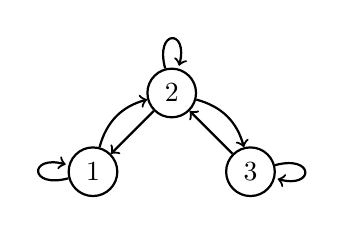
\begin{tikzpicture}
\begin{scope}[every node/.style={circle,thick,draw}]
    \node (A) at (0,0) {\m{1}};
    \node (B) at (1,1) {\m{2}};
    \node (C) at (2,0) {\m{3}};
\end{scope}
\begin{scope}[every edge/.style={draw=black,thick}]
    \path[->] (A) edge [loop left] (A)
                  edge [bend left] (B);
    \path[->] (B) edge [loop above] (B)
                  edge [bend left] (C)
                  edge [left] (A);
    \path[->] (C) edge [loop right] (C)
                  edge [left] (B);
\end{scope}
\end{tikzpicture}
\end{center}

Relacja ta jest zwrotna, jest symetryczna ale nie jest przechodnia. Powyższa relacja jest więc odpowiedzią. Zapiszmy tą relację jako zbiór par:

\[
    R = \{ \pair{1}{1}, \pair{1}{2}, \pair{2}{1}, \pair{2}{2}, \pair{2}{3}, \pair{3}{2}, \pair{3}{3} \} 
\]

Żeby sprawdzić, czy relacja jest rzeczywiście zwrotna, symetryczna i nie jest przechodnia, należy sprawdzić, czy dla każdego \m{a \in A} para \m{\pair{a}{a}} należy do zbioru \m{R} (zwrotność), czy dla każdej pary \m{\pair{a}{b}} należącej do \m{R}, para \m{\pair{b}{a}} też należy do \m{R} (symetryczność), oraz pokazać, że istnieją takie \m{a,b,c \in A}, że \m{\pair{a}{b} \in R} oraz \m{\pair{b}{c} \in R}, ale \m{\pair{a}{c} \not\in R} (przykładem takich \m{a, b, c} są kolejno \m{1,2,3}).

\end{example}
\begin{example}
Pokaż, że relacja \m{R \subseteq \mathbb{Q} \times \mathbb{Q}} jest zwrotna, symetryczna i przechodnia.

\[
 xRy \stackrel{def}{\Longleftrightarrow} \frac{x-y}{2} \in \mathbb{Z}
\]

Zacznijmy od pokazania, że relacja \m{R} jest \textbf{zwrotna}:

\begin{proof}
Relacja \m{R} jest zwrotna.

Żeby to pokazać, skorzystamy z definicji zwrotności. Przypomnijmy, że relacja jest zwrotna, jeśli dla każdego \m{a \in \mathbb{Q}}, zachodzi \m{aRa}, czyli, że \m{a} jest w relacji z \m{a}.

Weźmy więc dowolną liczbę wymierną \m{a}. Z definicji, \m{aRa} jeśli \m{\frac{a-a}{2} \in \mathbb{Z}}. Ale \m{\frac{a-a}{2} = \frac{0}{2} = 0}, i \m{0 \in \mathbb{Z}}, a to chcieliśmy pokazać.
\end{proof}

Wiemy już, że relacja jest zwrotna, pokażmy więc, że jest także symetryczna:

\begin{proof}
Relacja \m{R} jest symetryczna.

Żeby to pokazać, skorzystamy z definicji symetryczności. Przypomnijmy, że relacja jest symetryczna, jeśli dla dowolnych \m{a,b \in \mathbb{Q}}, zachodzi \m{aRb \Rightarrow bRa}, czyli jeśli \m{a} jest w relacji z \m{b}, to \m{b} jest w relacji z \m{a}.

Weźmy więc dowolne liczby wymierne \m{a,b} i załóżmy, że \m{aRb}, czyli, że \m{\frac{a-b}{2} = x} dla pewnej liczby całkowitej \m{x}. 

Pokażemy, że \m{bRa}, czyli, z definicji, że \m{\frac{b-a}{2} \in \mathbb{Z}}. Ale \m{\frac{b-a}{2} = -\frac{a-b}{2} = -x}. Skoro \m{x} było liczbą całkowitą, to \m{-x} także jest liczbą całkowitą, a to chcieliśmy pokazać.
\end{proof}

Do pokazania zostało nam że \m{R} jest przechodnia:

\begin{proof}
Relacja \m{R} jest przechodnia.

Żeby to pokazać, skorzystamy z definicji przechodniości. Przypomnijmy, że relacja jest przechodnia, jeśli dla dowolnych \m{a,b,c \in \mathbb{Q}} zachodzi \m{aRb \wedge bRc \Rightarrow aRc}, czyli jeśli \m{a} jest w relacji z \m{b} i \m{b} jest w relacji z \m{c}, to \m{a} jest w relacji z \m{c}.

Weźmy więc dowolne liczby wymierne \m{a,b,c} i załóżmy, że \m{aRb} i \m{bRc}, czyli, że \m{\frac{a-b}{2} = x} i \m{\frac{b-c}{2} = y} dla pewnych liczb całkowitych \m{x} oraz \m{y}.

Pokażemy, że \m{aRc}, czyli, z definicji, że \m{\frac{a-c}{2} \in \mathbb{Z}}. 
\[
 \frac{a-c}{2} = \frac{a-(b-b)-c}{2} = \frac{a-b+b-c}{2} = \frac{a-b}{2} + \frac{b-c}{2} = x + y
\]
Skoro \m{x} oraz \m{y} były liczbami całkowitymi, to \m{x+y} także jest liczbą całkowitą, a to chcieliśmy pokazać.
\end{proof}
\end{example}


\section{Złożenie relacji, relacja odwrotna}

\begin{definition}[Złożenie relacji]
Złożeniem relacji \m{P \subseteq A\times B} i \m{Q \subseteq B\times C} nazywamy relację 
\[
    P;Q = \set{\pair{a}{c}}{\exists{b}(aPb \wedge bQc)} \subseteq A\times C
\]
\end{definition}

Innymi słowy, \m{a \in A} i \m{c \in C} są w relacji \m{P;Q}, jeśli istnieje pewne ,,pośrednie'' \m{b \in B}, takie, że \m{a} jest w relacji \m{P} z \m{b} i \m{b} jest w relacji \m{Q} z \m{c}.

\begin{example}
\label{example:composition}
Niech \m{A = \{ 1,2,3 \}}, \m{B = \{ 4,5,6 \}} i \m{C = \{7,8 \}}. Dla relacji \m{P \subseteq A\times B} i \m{Q \subseteq B\times C} , zapisz relację \m{P;Q}.

\m{P = \{ \pair{1}{4},\pair{1}{6},\pair{3}{6},\pair{2}{5} \}} 

\m{Q = \{ \pair{4}{8}, \pair{6}{7}, \pair{5}{8} \}}
\[
 P;Q = \{ \pair{1}{8}, \pair{1}{7}, \pair{3}{7}, \pair{2}{8} \}
\]
\begin{itemize}
    \item Para \m{\pair{1}{8} \in P;Q}, bo \m{\pair{1}{4} \in P} i \m{\pair{4}{8} \in Q}.  
    \item Para \m{\pair{1}{7} \in P;Q}, bo \m{\pair{1}{6} \in P} i \m{\pair{6}{7} \in Q}.
    \item Para \m{\pair{3}{7} \in P;Q}, bo \m{\pair{3}{6} \in P} i \m{\pair{6}{7} \in Q}.
    \item Para \m{\pair{2}{8} \in P;Q}, bo \m{\pair{2}{5} \in P} i \m{\pair{5}{8} \in Q}.    
\end{itemize}

\end{example}

\begin{definition}[Relacja odwrotna]
Relacją odwrotną do relacji \m{P \subseteq A\times B} nazywamy relację 
\[
    P^{-1} = \set{\pair{b}{a}}{ \pair{a}{b} \in P } \subseteq B\times A
\]
\end{definition}

Innymi słowy, \m{b \in B} i \m{a \in A} są w relacji \m{P^{-1}}, jeśli \m{a} i \m{b} są w relacji \m{P}.

\begin{example}
Niech \m{A = \{ 1,2,3 \}} i \m{B = \{ 4,5,6 \}}. Dla relacji \m{P \subseteq A\times B}, zapisz relację \m{P^{-1}}.

\m{P = \{ \pair{1}{4},\pair{1}{6},\pair{3}{6},\pair{2}{5} \}} 
\[
 P^{-1} = \{ \pair{4}{1}, \pair{6}{1}, \pair{6}{3}, \pair{5}{2} \}
\]
\begin{itemize}
    \item Para \m{\pair{4}{1} \in P^{-1}}, bo \m{\pair{1}{4} \in P}.  
    \item Para \m{\pair{6}{1} \in P^{-1}}, bo \m{\pair{1}{6} \in P}.  
    \item Para \m{\pair{6}{3} \in P^{-1}}, bo \m{\pair{3}{6} \in P}.  
    \item Para \m{\pair{5}{2} \in P^{-1}}, bo \m{\pair{2}{5} \in P}.  
\end{itemize}

\end{example}

\section{Relacyjny rachunek dziedzin}

Relacyjny rachunek dziedzin jest jednym z języków zapytań, używanych w teorii \textbf{relacyjnych baz danych}, czyli baz danych, który opiera się na pojęciu \textbf{relacji}. Dane w takich bazach przedstawiane są za pomocą tabel (\textbf{relacji}) a ich zawartość wydobywa się za pomocą różnych języków zapytań, których przykładem może być omawiany w tym rozdziale \textbf{relacyjny rachunek dziedzin}. 

Relacyjny rachunek dziedzin używa pojęć, które poznaliśmy podczas omawiania zbiorów i relacji, a także z formuł rachunku kwantyfikatorów i jest używany w praktyce, do zapewnienia teoretycznych podstaw do relacyjnych baz danych.

Zapytania w tym języku są wyrażeniami w postaci

\[
    \set{\tuple{x_1, \dots, x_n}}{\varphi}
\]

Gdzie \m{\varphi} jest formułą rachunku kwantyfikatorów zawierająca zmienne wolne \m{x_1, \dots, x_n}. Jest to więc zbiór obiektów \m{x_1, x_2, \dots, x_n}, spełniających formułę \m{\varphi}. Zbiór takich obiektów czasem będziemy nazywać \textit{wykazem}. 

Dla przykładu \textit{,,wykaz studentów informatyki''}, dla zbioru wszystkich studentów \m{S}, kierunków \m{K} oraz relacji \m{Studiuje \subseteq S\times K}, można wyrazić zapytaniem \m{\set{x}{x \in S \wedge Studiuje(x,"Informatyka")}}.

W powyższym przykładzie warto zwrócić uwagę na \m{x \in S} -- musimy zapewnić, że obiekty są w rzeczywistości studentami, oraz na relację \m{Studiuje} -- ważna jest tu kolejność argumentów.

\begin{example}
\label{example:juices-and-bars}
Rozważmy zbiory osób \m{O}, barów \m{B} oraz soków \m{S} a także relacje \m{Bywa \subseteq O\times B}, \m{Lubi \subseteq O\times S} i \m{Podawany \subseteq S\times B}, informujące odpowiednio o tym, jakie osoby bywają w jakich barach, jakie osoby lubią jakie soki i jakie soki podawane są w jakich barach. W relacyjnym rachunku dziedzin wyraź poniższe zapytania:

\begin{itemize}
    \item Wykaz osób które nie bywają w żadnym barze, w którym podają sok ,,Malinowy''.
    
    Przypomnijmy, że zapytanie musi być w postaci \m{\set{x}{\varphi}}, gdzie \m{\varphi} jest formułą rachunku kwantyfikatorów zawierającą zmienną wolną \m{x}. 
    
    Formuła \m{\varphi} powinna opisywać zdanie \textit{,,\m{x} jest osobą, która nie bywa w żadnym barze, w którym podają sok malinowy''}. 
    
    Przede wszystkim więc musimy zapisać, że \m{x \in O}, to znaczy, że interesują nas tylko obiekty, które są osobami. Po drugie, \m{x} nie bywa w żadnym barze, w którym podają sok ,,Malinowy'', lub inaczej, w każdym barze, w którym \m{x} bywa, sok ,,Malinowy'' nie jest podawany, co możemy zapisać jako \m{\forall{b \in B} (Bywa(x,b) \Rightarrow \neg Podawany(''Malinowy'',b))}.
    
    Zauważmy, że w tej części zapytania jest \textit{implikacja}. Zazwyczaj po kwantyfikatorze ogólnym występuje właśnie implikacja. Gdybyśmy zamiast tego użyli koniunkcji, jeśli istniałby bar w którym \m{x} nie bywa, formuła byłaby fałszywa, zbiór byłby więc pusty. 
    
    Ostatecznie, nasze zapytanie w relacyjnym rachunku dziedzin przyjmuje postać:
    
    \[
        \set{x}{x \in O \wedge \forall{b \in B} (Bywa(x,b) \Rightarrow \neg Podawany(''Malinowy'',b))}
    \]
    
    \item Wykaz osób, które nie lubią żadnego soku, podawanego w barze ,,Jagoda''
    
    Ponownie, zapytanie musi być w postaci \m{\set{x}{\varphi}}.
    
    Formuła \m{\varphi} powinna więc opisywać zdanie \textit{,,\m{x} jest osobą, która nie lubi żadnego soku, podawanego w barze ,,Jagoda''}.
    
    Ponownie, pamiętać musimy o zapisaniu, że interesują nas tylko osoby: \m{x \in O}. Po drugie, zapisać musimy, że \m{x} nie lubi żadnego soku podawanego w barze ,,Jagoda'', lub inaczej, dla każdego soku podawanego w barze ,,Jagoda'', \m{x} go nie lubi: \m{\forall{s \in S} ( Podawany(s,''Jagoda'') \Rightarrow \neg Lubi(x,s))}.
    
    Ostatecznie, nasze zapytanie w relacyjnym rachunku dziedzin przyjmuje postać:

    \[
        \set{x}{x \in O \wedge \forall{s \in S} ( Podawany(s,''Jagoda'') \Rightarrow \neg Lubi(x,s))}
    \]
    
    \item Wykaz osób bywających w barze ,,Jagoda'', które lubią pewien podawany tam sok, którego nie lubi ,,Bartek''.
    
    Ponownie, zapytanie musi być w postaci \m{\set{x}{\varphi}}.
    
    Formuła \m{\varphi} powinna więc opisywać zdanie \textit{,,\m{x} jest osobą bywającą w barze ,,Jagoda'', która lubi pewien podawany tam sok, którego nie lubi ,,Bartek''}.
    
    Ponownie, pamiętać musimy o zapisaniu, że interesują nas tylko osoby: \m{x \in O}. Osoba \m{x} musi także bywać w barze ,,Jagoda'': \m{Bywa(x,''Jagoda'')}. Na koniec zapisać musimy, że w barze ,,Jagoda'' podają jakiś sok, lubiany przez \m{x}, którego nie lubi ,,Bartek'', lub inaczej, że istnieje sok, podawany w barze ,,Jagoda'', lubiany przez \m{x}, którego nie lubi ,,Bartek'': 
    
    \m{\exists{s \in S} (Podawany(s,''Jagoda'') \wedge Lubi(x,s) \wedge \neg Lubi(''Bartek'',s))}
    
    Warto zwrócić uwagę, że w tej części zapytania pojawiła się \textit{koniunkcja}. Zazwyczaj po kwantyfikatorze egzystencjalnym występuje właśnie koniunkcja.
    
    Ostatecznie, nasze zapytanie w relacyjnym rachunku dziedzin przyjmuje postać:
    
    \[
        \begin{split}
            \set{x}{&x \in O\ \wedge\\ 
            &Bywa(x,''Jagoda'')\ \wedge\\
            &\exists{s \in S}\ (Podawany(s,''Jagoda'') \wedge Lubi(x,s) \wedge \neg Lubi(''Bartek'',s)}
        \end{split}
    \]
    
\end{itemize}

Relacyjny rachunek dziedzin w dużej mierze opiera się na odpowiedniej interpretacji zdań w języku polskim, oraz umiejętnym zapisaniu ich w języku matematyki. Dla lepszego zrozumienia dobrze jest zadawać sobie pytania o przypadki brzegowe. Dla przykładu, \textit{,,co jeśli żadna osoba nie lubi żadnego soku''} lub, \textit{,,Co jeśli w barze \m{,,Jagoda''} nie podają żadnego soku}.
\end{example}

